%!TEX root = ./main.tex

\section{Quadratic optimization on the hypercube}

\subsection{Max-cut}

	In this subsection, let us describe how the content of the previous three subsections interact through an example, and give an approximation algorithm for the max-cut problem.

	\begin{question*}
		Given a graph $G = (V,E)$, find $S \subseteq V$ such that the size of the cut $E(S,S^c) = \left\{ \{i,j\} \in E : i \in S, j \in S^c \right\}$ is maximized.
	\end{question*}

	Unlike min-cut, which may be solved in polynomial time using flow, the above is \textsf{NP}-complete.

	One basic approximation algorithm was proposed by Erd\H{o}s, which merely returns a random cut. With constant probability, the returned cut is a $1/2$-approximation of the max-cut. We shall in this algorithm study an algorithm due to Goemans and Williamson \cite{gw-maxcut}.\\
	Assume wlog that $V = [n]$, and identify any $S \subseteq V$ with the vector in $\{-1,1\}^n$ with a $1$ at precisely those vertices in $S$. Note that the function defined by
	\[ f_G(x) = \frac{1}{4} \sum_{ij \in E} (x_i - x_j)^2 = \frac{1}{2} \sum_{ij \in E} (1 - x_ix_j). \]
	on input $S$ returns precisely the size of the cut corresponding to $S$. Equivalently, considering the \emph{graph Laplacian} $L_G \defeq D_G - A_G$, where $D_G$ is the diagonal matrix of degrees and $A_G$ is the adjacency matrix, we have
	\begin{equation}
		\label{eqn: gw-lapl}
		f_G(x) = \frac{1}{4} x^\top L_G x.
	\end{equation}
	We are interested in $\max_{x \in \{-1,1\}^n} f_G(x) \eqdef \opt(G)$.
	%Now, inspired by SDPs, consider the relaxation where instead of looking at $\langle L,xx^\top\rangle$, we look at $\frac{1}{4}\langle L,X\rangle$ together with the constraint that $X \pge 0$. We also fix the diagonal entries of $X$ to be $1$.

	\begin{ftheo}
		\label{theo: gw-sos}
		Set $\aGW \defeq \min_{\rho \in [-1,1]} \frac{2\arccos(\rho)}{\pi(1-\rho)} \approx 0.8786$. Then,
		\[ \frac{\opt(G)}{\aGW} - f_G(x) \ge 0 \]
		has a degree $2$ sum-of-squares certificate.
	\end{ftheo}

	Let $\pE_\opt$ be a pseudoexpectation that maximizes $\pE_\opt f_G$ as $\opt_{\text{SOS}_2}(G)$. Clearly, $\opt_{\SOS_2}(G) \ge \opt(G)$. Furthermore, by the previous theorem,
	\[ \opt(G) \le \opt_{\text{SOS}_2}(G) \le \frac{1}{\aGW} \opt(G). \]
	By the discussion at the end of the previous subsection, we can find in $\poly(n,1/\epsilon)$ a degree $2$ pseudodistribution $\mu$ such that
	\[ \pE_\mu f_G \ge \opt_{\text{SOS}_2}(G) - \epsilon. \]
	So,
	\[ \frac{1}{\aGW} \opt(G) \ge \pE_\mu f_G \ge \opt(G) - \epsilon. \]

	\begin{flem}
		\label{lem: gw-pd-to-rd}
		Let $\mu$ be a degree $2$ pseudodistribution on $\{-1,1\}^n$. Then, there exists a (``real'') distribution $\mu'$ on $\{-1,1\}^n$ such that
		\[ \E_{\mu'} f_G \ge \aGW \cdot \pE_{\mu} f_G. \]
	\end{flem}
	Further, it is possible to efficiently sample from $\mu'$ given $\mu$. Plugging this back into our previous sequence of equations,
	\[ \E_{\mu'} f_G \ge \aGW(\opt(G) - \epsilon) \ge (\aGW - \epsilon) \opt(G), \]
	and efficient sampling implies that we can in $\poly(n,1/\epsilon)$ time sample a random cut $S$ such that with good probability, the size of the cut of $S$ is a $(\aGW-\epsilon)$-approximation of the max-cut.\\
	Let us now get to the proofs of the above results.

	\begin{proof}[Proof that \Cref{lem: gw-pd-to-rd} implies \Cref{theo: gw-sos}]
		It suffices to show that for all pseudodistributions $\pE_\mu$,
		\[ \pE_\mu \left[ \frac{\opt(G)}{\aGW} - f_G \right] \ge 0. \]
		Equivalently, we would like to show that
		\[ \pE_\mu f_G \le \frac{\opt(G)}{\aGW}. \]
		Letting $\mu'$ be a distribution as in \Cref{lem: gw-pd-to-rd},
		\[ \pE_\mu f_G \le \frac{1}{\aGW} \E_{\mu'} f_G \le \frac{1}{\aGW} \opt(G). \qedhere \]
	\end{proof}

	\begin{proof}[Proof of \Cref{lem: gw-pd-to-rd}]
		We may assume wlog that $\pE_\mu x = 0$, by changing $\mu(x)$ to $\frac{\mu(x) + \mu(-x)}{2}$ -- note that this procedure does not change $\pE_\mu f_G$ because $f_G(x) = f_G(-x)$. Using \Cref{prop: pe-characterization}(b) and recalling that any principal submatrix of a PSD matrix is PSD, $\pE_\mu xx^\top \pge 0$. So, let $\nu$ be a normal distribution on $\R^n$ with mean $0$ and covariance matrix $\pE_\mu xx^\top$. Finally, define $\mu'$ by the process that samples a vector $g$ according to $\nu$ and returns $\hat{x} = \sign(g)$, the vector in $\{-1,1\}^n$ whose $i$th coordinate is just the sign $\pm 1$ of $g_i$ -- this is well-defined with probability $1$. Note that an $(x_i - x_j)^2$ term in $f_G$ contributes to the cut iff $\sign(g_i) \ne \sign(g_j)$. That is,
		% box-muller transform can be used to get the gaussian
		\[ \E_{\mu'} f_G = \sum_{ij \in E} \Pr[\sign(g_i) \ne \sign(g_j)]. \]
		For distinct $i,j$, set $\rho_{ij} = \E_{\mu}[x_i x_j] = \E [g_i g_j]$. Let $h \sim \mathcal{N}(0,\Id_2)$. Then, to analyze the above probability (for a fixed $i,j$), we can assume that $g_i = \langle h,v\rangle$ and $g_j = \langle h,w\rangle$ for some $v,w$ such that $\langle v,w\rangle = \rho_{ij}$. So, $\sign(g_i) \ne \sign(g_j)$ iff $\langle h,v\rangle$ and $\langle h,w\rangle$ have opposite signs. Because the ``direction'' $h/\|h\|$ of $h$ is uniformly distributed on $\mathbb{S}^1$, we get that
		\[ \Pr[\sign(g_i) \ne \sign(g_j)] = \frac{\arccos(\rho_{ij})}{\pi}, \]
		as seen in the following diagram, where $h$ must lie in the green region for the signs to be different.

		\begin{center}
		% \centering
		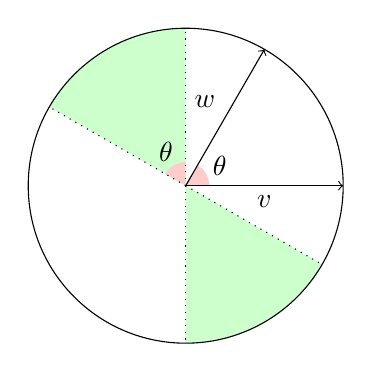
\begin{tikzpicture}
			\path[fill=green!20] (0,0) -- +(90:2) arc (90:150:2) -- (0,0);
			\path[fill=green!20] (0,0) -- +(-90:2) arc (-90:-30:2) -- (0,0);
			\coordinate (o) at (0,0);
			\coordinate (v) at (0:2);
			\coordinate (w) at (60:2);
	        \path[fill=red!20] (o) -- ++(60:.3) arc (60:0:.3) -- (o);
	        \path[draw] ++(30:.5) node {$\theta$};
	        \path[fill=red!20] (o) -- ++(90:.3) arc (90:150:.3) -- (o);
	        \path[draw] ++(120:.5) node {$\theta$};
	        \draw[dotted] (o) -- (90:2);
	        \draw[dotted] (o) -- (150:2);
	        \draw[dotted] (o) -- (-30:2);
	        \draw[dotted] (o) -- (-90:2);
			\draw[->] (0,0) coordinate (O) -- (0:2) coordinate (v) node[midway,below] {$v$};
			\draw[->] (0,0) coordinate (O) -- (60:2) coordinate (w) node[midway,above left] {$w$};
			\draw (0,0) circle (2 cm);
		\end{tikzpicture}

		The angle between $v,w$ is $\theta = \arccos(\rho_{ij})$.%\\So, $\Pr[\sign(\langle h,v\rangle) \ne \sign(\langle h,w\rangle)]$ is precisely $\theta/\pi$.
		\end{center}

		Using the facts that $\E[g_i^2] = 1$ and $\E[g_ig_j] = \rho_{ij}$, we have that $\E[(g_i - g_j)^2] = 2(1-\rho_{ij})$ and so
		\begin{align*}
			\E_{\mu'} f_G &= \sum_{ij \in E} \Pr[\sign(g_i) \ne \sign(g_j)] \\
				&= \sum_{ij \in E} \frac{\arccos(\rho_{ij})}{2\pi(1-\rho_{ij})} \E[(g_i - g_j)^2] \\
				&\ge \frac{\aGW}{4} \cdot \E\left[\sum_{ij \in E} (g_i - g_j)^2\right] = \aGW \pE_{\mu} f_G. \qedhere
		\end{align*}
	\end{proof}

	Now, we have managed to get roughly an $\aGW$-approximation using degree $2$ SoS. Is it possible to do any better using degree $2$ SoS? What about with a higher (but constant) degree? It might even be interesting to see if we can get a better approximation with non-constant degree, say $O(\log n)$.\\
	To answer the first question, it turns out that what we have done is indeed the best possible. A strong result regarding the constant degree case is due to Khot-Kindler-Mossel-O'Donnell \cite{max-cut-ugc}, where it is proved that Khot's \emph{Unique Games Conjecture} (UGC) \cite{ugc-og} implies that an $(\aGW+\epsilon)$-approximation is $\NP$-hard for any $\epsilon > 0$. While it is unknown at the time of writing this whether the unique games conjecture is true, we have strong reason to believe that it is due to a recent result \cite{2-2-gc} which proves the ``$2$-to-$2$ Games Conjecture'', a close variant of the unique games conjecture. We shall later look at the UGC in more detail.\\

	Let us get back to the Goemans-Williamson algorithm. Instead of looking at the best approximation ratio, can we parametrize the output result in terms of the optimal value?

	\begin{fprop}
		\label{prop: gw-reparametr}
		Let $G$ be a graph with $\opt(G) = (1-\delta)|E|$. For the output distribution $\mu'$ of the Goemans-Williamson algorithm, $\E_{\mu'} f_G = (1 - O(\sqrt{\delta})) |E|$.
	\end{fprop}
	\begin{proof}
		*** INCOMPLETE ***
	\end{proof}

	Is this rounding we have done, called ``Gaussian rounding'', the best possible? It turns out that it is not, and we can in general do better using the ``RPR$^2$'' scheme of roundings. We shall soon study this in more detail.\\

	Let us now return to our earlier statement that it is impossible to do better using degree $2$ SoS. That is, for graphs in general, if we can get a degree $2$ SoS certificate of non-negativity for
	\[ \frac{\opt(G)}{c} - f_G(x), \]
	how large can $c$ be? We shall show that $c = \aGW$ is optimal, by looking at the cycle $C_n$ for odd $n$. This serves as a ``gap'' example. It is easily seen that the max-cut in this graph is $n-1 = \left( 1 - \frac{1}{n} \right) |E|$. We shall show that there exists a degree $2$ pseudodistribution $\mu$ such that
	\[ \pE_\mu f_{C_n} \ge \left( 1 - O\left(\frac{1}{n^2}\right) \right) |E|. \]
	Due to \Cref{prop: gw-reparametr}, this shows that the Goemans-Williamson algorithm is tight, at least up to constant factors. We can think of the cycle as something of a discretization of the $2$-dimensional sphere. If we instead look at the discretization of a high-dimensional sphere, it can be shown that this is tight even up to constant factors. We refer the reader to \cite{gw-tight-feige-schechtman} for details. The sketch of the proof for the cycle is as follows.\\
	Recall \cref{eqn: gw-lapl}, so we are interested in $\max_{x \in \{-1,1\}^n} x^\top L_G x$. This is at most $\max_{x : \|x\|_2 = \sqrt{n}} x^\top L_G x = n\|L_G\|_2$, which can be computed in polynomial time. Now, how do we construct a pseudodistribution $\pE$ for the cycle as mentioned earlier? Note that a given $\pE$ is a well-defined degree $2$ pseudodistribution iff $\pE (1,x) (1,x)^\top$ is a PSD matrix with $1$s on the diagonal. Now,
	\begin{align*}
		\pE f_G(x) &= \pE x^\top L_G x \\
			&= \pE \langle L_G , xx^\top \rangle \\
			&= \left\langle L_G , \pE xx^\top \right\rangle.
	\end{align*}
	Observe that the top eigenvalue of $L_G$ is indeed $1 - O(1/n^2)$, and this eigenspace is $2$-dimensional. It turns out that for an appropriate choice of $v_1,v_2$ in this eigenspace, we can ensure that $v_1v_1^\top + v_2v_2^\top$ does have only $1$s on the diagonal (this is essentially a consequence of the fact that $\sin^2\theta+\cos^2\theta = 1$).

\subsection{The positive semidefinite case}

	In the previous subsection, we looked at $\max_{x \in \{-1,1\}^n} x^\top L_G x$, where $L_G$ is the (positive semidefinite) Laplacian of a graph. This is an example of quadratic optimization, where we are more generally interested in
	\[ \opt(B) \defeq \max_{x \in \{-1,1\}^n} x^\top B x \]
	for some $n \times n$ matrix $B$.\\
	In the case where $B \pge 0$, it turns out that we can do something similar to what we had done in the max-cut algorithm.
	% -- it is possible to get a $\pi/2$-approximation, due to Nesterov \cite{quad-optim-psd}.

	\begin{ftheo}[Nesterov]
		\label{thm: nesterov}
		Let $B$ be a positive semidefinite $n\times n$ matrix. Then,
		\[ \frac{\opt(B)}{c} - x^\top B x \]
		has a degree $2$ sum-of-squares certificate for $c = 2/\pi \approx 0.63$.
	\end{ftheo}
	By the discussion in the previous section, this means as a corollary that we have a $\poly(n,1/\epsilon)$-time $(2/\pi-\epsilon)$-approximation algorithm for any $\epsilon > 0$.

	\begin{definition}
		Let $M \in \R^{n \times n}$. Given $f : \R \to \R$, define $f[M] \in \R^{n \times n}$ by $f[M]_{ij} = f(M_{ij})$ for all $i,j$.
	\end{definition}

	\begin{fprop}
		\label{prop: taylor-fM-psd}
		Suppose $M$ is a positive semidefinite matrix and $f$ a function whose Taylor series has all positive Taylor coefficients and is uniformly convergent on $[-1,1]$. Then, $f[M]$ is positive semidefinite.
	\end{fprop}

	The above is a corollary of the following simple observation.

	\begin{prop}[Schur Product Theorem]
		\label{schur-prod-thm}
		Let $M,M'$ be positive semidefinite matrices. Denote by $M \circ M'$ the \emph{Hadamard product} of $M,M'$ defined by $(M\circ M')_{ij} = M_{ij} M'_{ij}$. Then, $M \circ M'$ is positive semidefinite.
	\end{prop}
	\begin{proof}
		Let $M = \sum_i \lambda_i v_i v_i^\top$ and $M' = \sum_j \lambda_j' v_j'v_j'^\top$. Using linearity of the Hadamard product,
		\[ M \circ M' = \sum_{i,j} \lambda_i \lambda'_j (v_i v_i^\top) \circ (v_j v_j'^\top) = \sum_{i,j} \lambda_i \lambda'_j (v_i \circ v_j') (v_i \circ v_j')^\top \pge 0. \qedhere \]
	\end{proof}

	\begin{proof}[Proof of \Cref{prop: taylor-fM-psd}]
		Denote $[M]^2 = M \circ M$, and $[M]^i = [M]^{i-1} \circ M$ more generally. By the \nameref{schur-prod-thm}, $[M]^i \pge 0$ for all $i$. Therefore, $\sum c_i [M]^i \pge 0$, that is, $(\sum c_i x^i)[M] \pge 0$.
	\end{proof}

	% A straightforward corollary of \Cref{prop: taylor-fM-psd} is that $\arcsin[M] \pge M$.

	\begin{proof}[Proof of \nameref{thm: nesterov}]
		As in the previous subsection, let $\mu$ be a zero mean degree $2$ pseudodistribution on $\{-1,1\}^n$, $g$ a normal random variable with zero mean and covariance matrix $\pE_\mu xx^\top$, and $\hat{x} \defeq \sign(g)$ distributed as $\mu'$. A straightforward byproduct of the final part of the proof of \Cref{lem: gw-pd-to-rd} is that
		\[ \E_{\mu'}[\hat{x}_i \hat{x}_j] = \frac{2}{\pi} \arcsin\E[g_ig_j]. \]
		Therefore,
		\begin{align*}
			\E_{\mu'} \hat{x}^\top B \hat{x} &= \sum_{i,j} B_{ij} \E[\hat{x}_i \hat{x}_j] \\
				&= \sum_{i,j} B_{ij} \frac{2}{\pi} \arcsin[g_i g_j] \\
				&= \frac{2}{\pi} \left\langle B , \arcsin\left[\E gg^\top\right] \right\rangle.
		\end{align*}
		Recall that if $B,C \pge 0$, then $\langle B,C\rangle \ge 0$. In particular,
		\[ \left\langle B , \arcsin\left[\E gg^\top\right] - \E gg^\top \right\rangle \ge 0, \]
		so
		\[ \E_{\mu'} \hat{x}^\top B \hat{x} \ge \frac{2}{\pi} \langle B,\E gg^\top\rangle = \frac{2}{\pi} \pE_\mu x^\top B x. \]
		The remainder of the proof is identical to that in the previous subsection.
	\end{proof}

	% IS THIS TIGHT?


\subsection{The most general case}

	Let us next look at the case where $B$ is any arbitrary matrix. First of all, we may assume that $B$ is symmetric by looking at its symmetrization $(B+B^\top)/2$ instead.
	We may also assume that all diagonal entries of $B$ are $0$, since if we set $B = D + N$ where $D$ is diagonal and $N$ has all diagonal entries zero,
	\[ \max_{y \in \{-1,1\}^n} y^\top B y = \Tr(B) + \max_{y \in \{-1,1\}^n} y^\top N y. \]
	We assume so for the remainder of this subsection.\\
	We shall give an $O(\log n)$-approximation algorithm. First of all, is $\opt(B)$ even non-negative?

	\begin{fprop}
		\label{prop: solid-to-discrete-hypercube}
		Let $y \in [-1,1]^n$. Then, there exists $\hat{y} \in \{-1,1\}^n$ such that $\hat{y}^\top B y \ge y^\top B y$.
	\end{fprop}
	In particular, setting $y = 0$ implies that the desired value is non-negative.
	\begin{proof}
		Consider the random variable $\hat{y}$ on $\{-1,1\}^n$ which has $\hat{y}_i = 1$ with probability $(1+y_i)/2$ and $0$ with probability $(1-y_i)/2$, independently for different coordinates $i$. Note that $\E \hat{y}_i \hat{y}_j = y_i y_j$ for distinct $i, j$. Consequently,
		\[ \E_\mu \hat{y}^\top B \hat{y} = y^\top B y, \]
		so the desideratum follows.
	\end{proof}
	The above result is also true in the more general case where $\Tr(B) \ge 0$, but we do not require it.\\

	We can in fact get a stronger lower bound than just the $0$ in the above proposition.

	\begin{fprop}
		\[ \max_{y \in \{-1,1\}^n} y^\top B y \ge \frac{1}{n} \sum_{i,j} |B_{ij}|. \]
	\end{fprop}
	\begin{proof}
		*** INCOMPLETE ***
	\end{proof}

	The sum-of-squares proof we shall give is due to \cite{quad-optim-meg01,quad-optim-charikar-wirth}.

	\begin{ftheo}
		For sufficiently large $n$ and $c = O(\log n)$,
		\[ \frac{\opt(B)}{c} - x^\top B x \]
		has a degree $2$ sum-of-squares certificate.
	\end{ftheo}
	While we do not compute the exact constants exactly, the above is true for roughly $n > 60$ and $c = 4 \log n$.
	\begin{proof}
		As in the max-cut and PSD cases, we prove that given any pseudodistribution $\mu$, there exists an (efficiently sampleable) distribution $\mu'$ on $\{-1,1\}^n$ such that $\E_{\mu'} \hat{x}^\top B \hat{x} \ge \frac{1}{O(\log n)} \pE_\mu x^\top B x$. By \Cref{prop: solid-to-discrete-hypercube}, it suffices to show this for a distribution on the continuous hypercube $[-1,1]^n$ instead of $\{-1,1\}^n$.\\
		As before, choose $g \sim \mathcal{N}(0,\E_\mu xx^\top)$, so
		\[ \E[g^\top B g] = \pE_\mu [x^\top Bx]. \]
		Make the mild assumption that $\E[g^\top B g] \ge 0$; the analysis of the general case is nearly identical. For a suitable constant $C$, we have that
		\begin{align}
			\Pr[\|g\|_\infty > C \log n] \cdot \E[g^\top B g \mid \|g\|_\infty > C \log n] &\le \frac{1}{n^2} \E[g^\top B g] \text{, so} \nonumber \\
			\Pr[\|g\|_\infty \le C \log n] \cdot \E[g^\top B g \mid \|g\|_\infty \le C \log n] &\ge \left( 1 - \frac{1}{n^2} \right) \E[g^\top B g] \label{eqn: nesterov1}
		\end{align}
		Our assumption that $\E[g^\top B g] \ge 0$ also implies that all the quantities above are non-negative.
		The final random variable $\hat{x}$ on the solid hypercube is defined by
		\[ \hat{x}_i = \begin{cases} \frac{g_i}{C\sqrt{\log n}}, & |g_i| \le C\sqrt{\log n}, \\ \frac{g_i}{|g_i|}, & \text{otherwise.} \end{cases} \]
		Then,
		\begin{align*}
			\E[\hat{x}^\top B x] &\ge \Pr[\|g\|_\infty \le C\sqrt{\log n}] \cdot \E[\hat{x}^\top B \hat{x} \mid \|g\|_\infty \le C\sqrt{\log n}] \\
				&\ge \frac{1}{2C^2\log n}\E[g^\top B g \mid \|g\|_\infty \le C\sqrt{\log n}] \\
				&\stackrel{\eqref{eqn: nesterov1}}{\ge} \frac{1}{O(\log n)} \E[g^\top B g] = \frac{1}{O(\log n)} \pE_{\mu}[x^\top B x],
		\end{align*}
		completing the proof.
	\end{proof}

	This above rounding is a specific case of the more general RPR$^2$ scheme of roundings that we mentioned earlier. In this, we ``modify'' $\pE_\mu xx^\top$ in some way (in the above method of Nesterov, we scale it down), sample a Gaussian with this modified covariance matrix, then do randomized rounding. In the setting of max-cut, we search over all RPR$^2$ roundings and output whichever returns the maximum cut value.

\subsection{The bipartite support case}

	In this section, we shall look at the specific case where the \emph{support} $\supp(B) \defeq \{ \{i,j\} : B_{ij} \ne 0\}$ defines a bipartite graph (on vertex set $[n]$). We also assume that $B$ is symmetric by symmetrizing it. The constant-factor approximation we shall describe is due to Alon and Naor \cite{grothendieck-alon-naor}.

	Since $\supp(B)$ is bipartite, there exists some bipartition $X \cup Y$ of $[n]$ such that $B_{xx'} = B_{yy'} = 0$ for any $x,x' \in X$ and $y,y' \in Y$. Letting $B'$ be the submatrix of $B$ consisting of the $X$-rows and $Y$-columns (note that the submatrix consisting of the $Y$-rows and $X$-columns is then $B'^\top$) and splitting a given vector $x \in \R^{n}$ into two parts $(x_X,x_Y)$, we have that
	\[ x^\top B x = 2x_X^\top B' x_Y. \]
	Therefore, our optimization problem is equivalent to the following: given an arbitrary $n \times n$ matrix $B$, determine
	\[ \max_{x,y \in \{-1,1\}^n} x^\top B y. \]
	For simplicity, denote the above maximum by $\opt(B)$.\\

	While the $B'$ we looked at above in the bipartite setting need not be square, we can assume it is by appending appropriately many rows/columns filled with zeros.\\
	Given norms ${\color{red}{\|}}\cdot{\color{red}{\|}}$ and ${\color{olive}{\|}}\cdot{\color{olive}{\|}}$ on $\R^n$, we have an associated \emph{operator norm} on matrices defined by
	\[ {\color{red}{\|}}A{\color{olive}{\|}} = \inf\{c \ge 0 : {\color{red}{\|}}Ax{\color{red}{\|}} \le {\color{olive}{\|}}x{\color{olive}{\|}} \text{ for all }x\in\R^n \}. \]
	When the first norm is the $L^p$ and the second is the $L^q$, the operator norm is denoted the $\|\cdot\|_{q \to p}$ norm. That is,
	\[ \|A\|_{q \to p} \defeq \max_{\substack{x \in \R^n \\ x \ne 0}} \frac{\|Ax\|_p}{\|x\|_q}. \]
	Now, note that for a given $x$,
	\[ \max_{y \in \{-1,1\}^n} x^\top B y = \max_{y \in \{-1,1\}^n} \langle Bx , y\rangle = \|Bx\|_1, \]
	since we can just choose the sign of $y_i$ opposite to that of $(Bx)_i$. Further,
	\begin{align*}
		\|B\|_{\infty \to 1} &= \max_{\|x\| \le 1} \sum_i \left|\sum_j B_{ij} x_j\right| \\
			&= \max_{|x_i| = 1} \left|\sum_j B_{ij} x_j\right| \\
			&= \max_{x \in \{-1,1\}^n} \|Bx\|_1 = \max_{x,y \in \{-1,1\}^n} x^\top B y,
	\end{align*}
	where the second equality is because the summation is a convex function of the $(x_i)$, so it is maximized at a vertex of the cube $[-1,1]^n$, namely at a point in $\{-1,1\}^n$.
	Therefore, our problem is equivalent to approximating $\|B\|_{\infty \to 1}$ for an arbitrary matrix $B \in \R^{n \times n}$.

	\begin{ftheo}
		There exists a constant $K_G$ such that
		\[ K_G \opt(B) - x^\top B y \]
		has a degree $2$ sum-of-squares certificate.
	\end{ftheo}
	Interestingly, the exact value of $K_G$ is an open problem, and the interested reader may look up \emph{Grothendieck's inequality} for more details. It is known that
	\[ 1.57 \approx \frac{\pi}{2} \le K_G \le \frac{\pi}{2\ln(1+\sqrt{2})} \approx 1.78. \]
	We shall give a proof due to Krivine in 1977 which yields the bound on the right.

	\begin{proof}
		This proof is slightly different from previous ones in terms of execution. We shall show that given a degree $2$ pseudodistribution $\mu$ (on $\{-1,1\}^n$), there exists a real distribution $\mu'$ such that
		\[ \E_{\mu'} \hat{x} \hat{y}^\top = \frac{2\ln(1+\sqrt{2})}{\pi} \pE_\mu x y^\top. \]
		Given this,
		\begin{align*}
			\E_{\mu'} \hat{x}^\top B \hat{y} &= \left\langle B , \E_{\mu'} \hat{x} \hat{y}^\top \right\rangle \\
				&= \frac{2\ln(1+\sqrt{2})}{\pi} \left\langle B , \pE_{\mu} xy^\top \right\rangle = \frac{2\ln(1+\sqrt{2})}{\pi} \pE_\mu x^\top B y,
		\end{align*}
		so we are done by methods similar to previous proofs.
		We shall first modify the ``covariance matrix'' of $\pE$ in some manner to get another matrix $M'$ before creating the Gaussian used in rounding. Let $c = \ln(1+\sqrt{2})$. This matrix $M'$ is defined by
		\[ M' = \begin{pmatrix} \sinh\left[ c \pE_\mu xx^\top \right] & \sin\left[ c \pE_\mu xy^\top \right] \\ \sin\left[ c \pE_\mu yx^\top \right] & \sinh\left[ c \pE_\mu yy^\top \right] \end{pmatrix}. \]
		We shall explain the reasoning behind this choice in the proof.
		Then, we choose Gaussians $g,h \sim \mathcal{N}(0,M')$, and we finally define $\hat{x} = \sign(g)$ and $\hat{y} = \sign(h)$. To complete the proof, we need to show three things.
		\begin{enumerate}[label=(\alph*)]
			\item $\E_{g,h} \hat{x} \hat{y}^\top = (2c/\pi) \pE_{\mu} xy^\top$. Recall that
			\[ \E\hat{x} \hat{y}^\top = \frac{2}{\pi} \arcsin[\E gh^\top].  \]
			We want this expression on the left to be some constant times $\pE_\mu xy^\top$. So, it makes sense to choose $\E gh^\top = \sin[c \pE_\mu xy^\top]$. This means that the bottom-left and bottom-right of our modified matrix should look like that of $M'$. While this might inspire us to choose $\sin$s on the diagonal blocks as well, doing so causes problems when it comes to PSD-ness, so we choose $\sinh$ instead. The reason for the precise choice of $\sinh$ is explained when we look at why $M' \pge 0$.\\
			Recalling the definition of $\E gh^\top$ from $M'$,
			\[ \E[\hat{x} \hat{y}^\top] = \frac{2}{\pi} \arcsin[\E gh^\top] = \frac{2}{\pi} \arcsin[\sin[c \pE_\mu xy^\top]] = \frac{2\ln(1+\sqrt{2})}{\pi} \pE_\mu xy^\top. \]
			\item $M' \pge 0$. We saw earlier in the proof of \Cref{prop: taylor-fM-psd} that if $M$ is PSD, so is $[M]^i$. It turns out, in fact, that if
			\[ M = \begin{pmatrix} M_{11} & M_{12} \\ M_{21} & M_{22} \end{pmatrix} \]
			is PSD, so is
			\[ \begin{pmatrix} [M_{11}]^i & -[M_{12}]^i \\ -[M_{21}]^i & [M_{22}]^i \end{pmatrix}. \]
			Indeed,
			\[ \begin{pmatrix} v \\ w \end{pmatrix}^\top \begin{pmatrix} [M_{11}]^i & -[M_{12}]^i \\ -[M_{21}]^i & [M_{22}]^i \end{pmatrix} \begin{pmatrix} v \\ w \end{pmatrix} = \begin{pmatrix} v \\ -w \end{pmatrix}^\top \begin{pmatrix} [M_{11}]^i & [M_{12}]^i \\ [M_{21}]^i & [M_{22}]^i \end{pmatrix} \begin{pmatrix} v \\ -w \end{pmatrix} \]
			and the matrix on the right is PSD.
			Recalling that the Taylor series expansions of $\sin$ and $\sinh$ are given by
			\begin{align*}
				\sinh(x) &= \sum_{n=0}^{\infty} \frac{1}{(2n+1)!} x^{2n+1} \text{ and} \\
				\sin(x) &= \sum_{n=0}^{\infty} \frac{(-1)^n}{(2n+1)!} x^{2n+1},
			\end{align*}
			it follows by a proof very similar to that of \Cref{prop: taylor-fM-psd} that $M' \pge 0$.
			\item $M'_{ii} = 1$ for each $i$. The value of $c$ is forced by this requirement, and indeed $\sinh(\ln(1+\sqrt{2})) = 1$. \qedhere
		\end{enumerate}
	\end{proof}

	Krivine conjectured in his original paper that $K_G$ is exactly equal to this quantity. Later however, it was shown \cite{braverman-krivine} that $K_G$ is strictly less than this.